\chapter{Mathematical foundations}

\section{Probability theory}
Homomorphic encryption schemes are based on noise. As we will see in Subsection \ref{subsec:LWE}, noise can be sampled from discrete spaces in accordance with a distribution. Since distributions are central in cryptography, it is important they are understood. A distribution is a probability measure on a measurable space $(S, \mathcal{S})$. Typically, probability distributions are associated with random variables; however, in the absence of random variables, distributions are understood as a specified measure function on the given measurable space (See \cite[pp. 83]{kallenberg-probability}).
\begin{definition}[Discrete distribution measure of a random variable]
Consider a probability space $(\Omega, \mathcal{F}, \operatorname{Pr})$ and a discrete measurable space $(S,\mathcal{S})$. Let $X \colon \Omega \mapsto S$ be a random variable. The discrete distribution measure of $X$, or simply \emph{distribution} of $X$, $\chi$ is defined as follows
\begin{equation*}
\begin{aligned}
    \chi \colon \mathcal{S} &\to [0,1]\\
    \{x\} &\mapsto \operatorname{Pr}[X = x]
\end{aligned}
\end{equation*}
We say that $\chi$ is the distribution or \emph{law} of $X$, denoted $\mathcal{L}(X)$. 
\end{definition}
\begin{remark}
    Since $\chi$ is a measure on a discrete space, the description of the singletons are sufficient. More explicitly, $\chi(A) = \sum_{x \in A} \operatorname{Pr}[X = x]$ for $A \in \mathcal{S}$
\end{remark}
A distribution measure for a random variable is a probability measure on the sample space $(S,\mathcal{S})$, as opposed to on the outcome space $(\Omega, \mathcal{F})$. For a given probability space, any random variable $X$ defined on it has a distribution associated with it. We write $x \leftarrow X$ or $x \leftarrow \chi$ for sampling the outcome $x$ from $X$ assuming $\chi$ is its distribution. When $X$ is a space we mean that $x$ is uniformly sampled from $X$.

\begin{definition}[Ensembles] \label{def:prob-ensemble}
    Let $I$ be a countable index set. A \emph{probability ensemble} indexed by $I$ (or just ensemble) is a sequence of random variables $(X_i)_{i \in I}$. A \emph{distribution ensemble} indexed by $I$ is a sequence of distributions $(\chi_i)_{i \in I}$
\end{definition}
In this paper we will exclusively use $\mathbb{N}$ as the index set.
For example, the encryption function is a random variable (PPT algorithm), meaning that a single message $m$ corresponds to many valid ciphertexts. By varying the security parameter of the scheme we construct the probability ensemble $\{Enc(pk,m)\}_{pk \in \mathbb{N}}$
\begin{definition}[Statistical distance] \label{def:statistical-distance}
    Let $S_n$ be finite set for all $n \in \mathbb{N}$ and let $X = (X_n \colon \Omega_n \to S_n)_{n \in \mathbb{N}}$, $Y = (Y_n \colon \Omega_n \to S_n)_{n \in \mathbb{N}}$ be two ensembles. The \emph{statistical distance} is defined as
    \begin{equation*}
        \Delta_{X,Y}(n) \stackrel{\mathrm{def}}{=} \frac{1}{2} \sum_{\alpha \in S_n} |\operatorname{Pr}[X_n = \alpha] - \operatorname{Pr}[Y_n = \alpha]|.
    \end{equation*}
    Let $\chi = \{\chi_n\}_{n \in \mathbb{N}}$, $\psi = \{\psi_n\}_{n \in \mathbb{N}}$ be two discrete distribution ensembles on the same measurable spaces $\{(S_n, \mathcal{S}_n)\}_{n \in \mathbb{N}}$. The statistical distance is defined as
    \begin{equation*}
    \begin{aligned}
        \Delta_{\chi, \psi}(n) \stackrel{\mathrm{def}}{=} \frac{1}{2} \sum_{\alpha \in S_n} |\chi_n(\{\alpha\}) - \psi_n(\{\alpha\})|
    \end{aligned}
    \end{equation*}
\end{definition}
\begin{remark}
    This definition for distribution ensembles assumes every singleton is measurable. A more general definition is $\Delta(\chi, \psi) \stackrel{\mathrm{def}}{=} \sup _{A \in \mathcal{S}}|\chi(A)-\psi(A)|$ 
\end{remark}

\begin{definition}[Negligible function]
    Let $f \colon \mathbb{N} \to [0,1]$. $f$ is negligible if for all positive polynomials $p(\cdot)$, there exists an $N$ such that for all $n>N$, $f(n) < \frac{1}{p(n)}$. We say $f = \operatorname{negl}(n)$.
\end{definition}
\begin{definition}[Perfectly indistinguishable] \label{def:perfectly-indistinguishable}
    Two ensembles (probability or distribution) $X$ and $Y$ are \emph{perfectly indistinguishable} if $\Delta_{X,Y}(n) = 0$ for all $n$.
\end{definition}
\begin{definition}[Statistically indistinguishable] \label{def:statistically-indistinguishable}
    Two ensembles (probability or distribution) $X$ and $Y$ are \emph{statistically indistinguishable} if $\Delta_{X,Y}(n) = \operatorname{negl}(n)$.
\end{definition}
 A desirable property of encryption schemes is to make it unfeasible for adversaries to distinguish encryptions. For two random variables (or distributions) $X$ and $Y$, we want every adversary $C$ to not be able to distinguish samples from $X$ and $Y$. More precisely, an adversary tasked with identifying whether given samples are from $X$ ($C$ outputs 0) or from $Y$ ($C$ outputs 1) should have roughly the same probability of success irrespective of which the samples are generated from. The formal definition is as follows:\\\\\\\\
\begin{definition}[Computationally indistinguishable \cite{Gol01}] \label{def:computationally-indistinguishable}
    Two ensembles (or distribution ensembles) $X$ and $Y$ are computationally indistinguishable if, for every polynomial-size circuit family $C = \{C_n\}_{n \in \mathbb{N}}$, $$\operatorname{Adv}_{X,Y}(n) \stackrel{\mathrm{def}}{=} |\operatorname{Pr}[C(X_n) = 1] - \operatorname{Pr}[C(Y_n) = 1]| = \operatorname{negl}(n).$$
\end{definition}
$C(X_n), C(Y_n)$ means that the adversary has access to random oracle returning a sample from $X_n$ and $Y_n$ respectively. The point is that, for every adversary $C$ guessing the samples are from one of the random variables or distributions (1 in this case represents from $Y_n$), the probability of being correct is, up to negligible error, equal to the probability of being incorrect. For example, an adversary always guessing 1 has 100\% probability of being incorrect when given samples from $X_n$ and 100\% probability of being correct when given samples from $Y_n$. The intuition is that the sample does not make a noticable difference on the guess and that the advantage in distinguishing samples goes to zero fast (faster than the inverse of all polynomials).

Perfect distinguishability implies statistical indistinguishability as 0 is negligible. Statistical indistinguishability implies computational indistinguishability. To see why, assume $\Delta_{X,Y}(n) = \operatorname{negl}(n)$ and consider any circuit family $C$. Since $X_n$ and $Y_n$ are defined on the same space we have
\begin{equation*}
\begin{aligned}
    \operatorname{Adv}_{X,Y}(n) &= |\operatorname{Pr}[C(X_n) = 1] - \operatorname{Pr}[C(Y_n) = 1]|\\
        &\leq \sum_{\alpha \in S_n} | \operatorname{Pr}[C(X_n = \alpha) = 1 \; | \; X_n = \alpha]\operatorname{Pr}[X_n = \alpha] \\
        &\phantom{=} \qquad - \operatorname{Pr}[C(Y_n = \alpha) = 1 \; | \; Y_n = \alpha]\operatorname{Pr}[Y_n = \alpha] | \\
        &\leq \sum_{\alpha \in S_n} | \operatorname{Pr}[X_n = \alpha] - \operatorname{Pr}[Y_n = \alpha]| = 2\Delta_{X,Y}(n) = \operatorname{negl}(n)
\end{aligned}
\end{equation*}
where the first inequality is due to the triangle inequality and the second is due to conditional probability being upper bounded by 1. Intuitively, there does not exist enough distinguishable outcomes to distinguish the ensembles even if there exists an adversary that always correctly recognize an outcome from $X$ and $Y$ respectively.

\section{Distributions}
When working over integer lattices, the errors need to be sampled from discrete distributions. Furthermore, the desire is to keep the errors small. In this section we introduce the discrete Gaussian distribution, which is the most common distribution used in lattice-based cryptography. We also introduce subgaussian distributions, which are used in the error analysis of the GSW scheme in Chapter \ref{ch:implementation}.



\section{Discrete Gaussian Distribution}
To add discrete noise to ciphertexts, it is typical to use the discretized Gaussian distribution introduced by Micciancio and Regev \cite{disc-gauss}. Since this distribution is used so frequently, we give a brief presentation of it here. A continuous Gaussian distribution in $\mathbb{R}^n$ centered at $\vec{c}$ where each coordinate is independently sampled from normal distirbution with standard deviation $\sigma$, then the multivariate Gaussian distribution is simplified to $\rho_{\vec{c}}(\vec{x}; \sigma)=\frac{1}{\left(2 \pi \sigma^2\right)^{n / 2}} \exp \left( -\frac{1}{2 \sigma^2} \| \vec{x}-\vec{c} \| ^2\right)$. By introducing the scale factor $s \stackrel{\mathrm{def}}{=} \sqrt{2\pi}\sigma$ we get $\rho_{s, \vec{c}}(\vec{x})=\frac{1}{s^n} \exp \left(-\frac{\pi}{s^2} \| \vec{x}-\vec{c} \| ^2\right)$.
The goal is to discretize the Gaussian over lattices, see Section \ref{sec:hard_problems}, by restricting the domain to lattice points. For a given lattice $L \subset \mathbb{R}^n$ we define the normalization constant $\rho_{s, \vec{c}}(L) \stackrel{\mathrm{def}}{=} \sum_{\vec{x} \in L} \rho_{s, \vec{c}}(\vec{x})$.
\begin{definition}[Discrete Gaussian distribution]\label{Disc-Gauss}
    Let $L \subset \mathbb{R}^n$ be a lattice. Then the discrete Gaussian distribution is defined as
    \begin{equation*}
        \forall \vec{x} \in L \colon \quad \textrm{D}_{L, s, \vec{c}}(\vec{x}) \stackrel{\mathrm{def}}{=} \frac{\rho_{s, \vec{c}}(\vec{x})}{\rho_{s, \vec{c}}(L)}.
    \end{equation*}            
\end{definition}
\begin{definition}[$\beta$-bounded distribution]
    Let $\chi$ be a distribution over the integers. $\chi$ is $\beta$-bounded if $x \leftarrow \chi \implies |x| < \beta$
\end{definition}
\begin{remark}
    It is also possible (and common) to define a $\beta$-bounded distribution such that $|x| \geq \beta$ with negligible probability.
\end{remark}
\begin{figure}
    \centering
    \hypertarget{fig:discrete-gauss}{}
    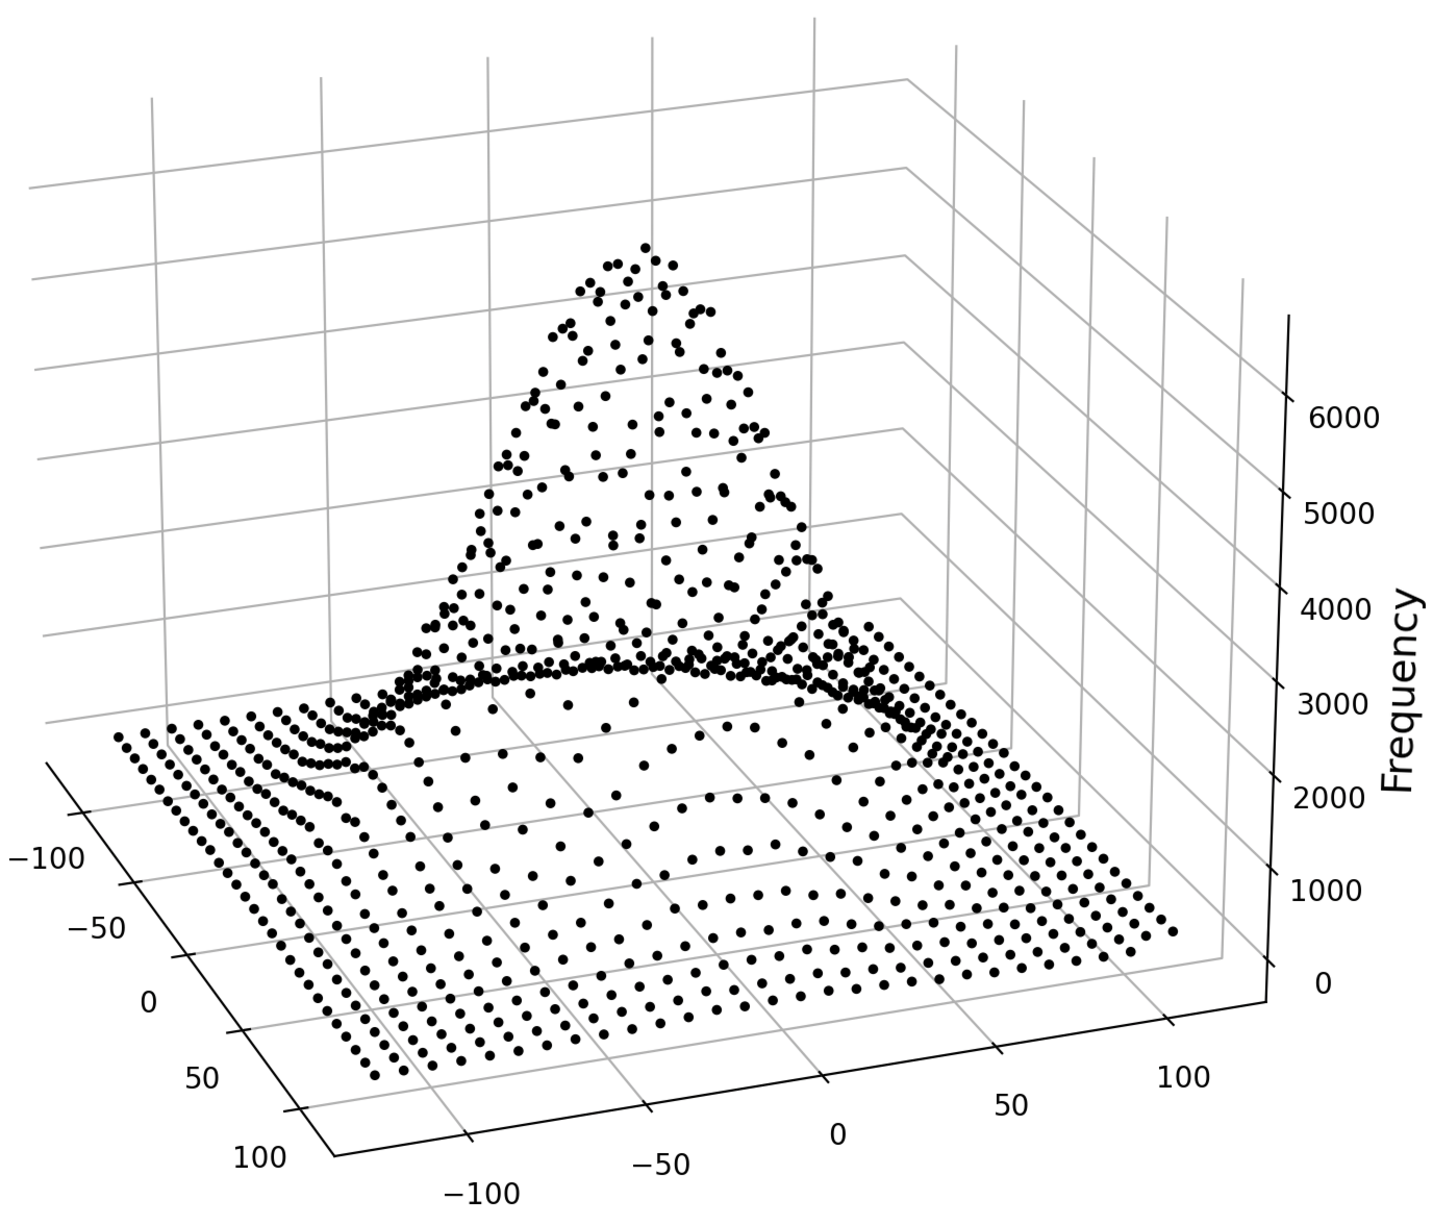
\includegraphics[width=0.65\textwidth]{figures/D-G-2d-a_is_100-n_1000000.pdf}
    \caption*{\textbf{Figure 1}: Discrete Gaussian distribution $\textrm{D}_{\mathbb{Z}^2, 100, \vec{0}}$ with 1 million samples. Every point has integer coordinates. See code in Appendix \ref{app:code}.}
\end{figure}

\subsection*{Subgaussian distributions}
In this section we introduce subgaussian distributions. We use subgaussian distributions for a tighter error analysis when discussing the GSW scheme in Chapter \ref{ch:implementation}. Much of this section can be found in \cite{A-S-P-boot}.
\begin{definition}[Subgaussian distribution]
    A distribution $\chi$ over $\mathbb{R}$ is subgaussian with parameter $K > 0$ ($K$ not nesessarily constant) if for every non negative $t \in \mathbb{R}$.
    \begin{equation*}
        \chi(\{x \in \mathbb{R} \text{ such that} \; |x| > t\}) \leq 2\exp \left(- \pi \frac{t^2}{K^2} \right)
    \end{equation*}
    Or equivalently, a real valued random variable $X$ has subgaussian distribution if
    \begin{equation*}
        \operatorname{Pr}[|X|>t] \leq 2\exp \left(- \pi \frac{t^2}{K^2} \right)
    \end{equation*}
    We say $X$ is a subgaussian random variable.
\end{definition}
The intuition of subgaussian distributions is that the probability of a random variable $X$ taking a large value is less than the probability of a Gaussian taking the same value. In other words, the tails of a subgaussian distribution decays at least as fast as the tails of a Gaussian distribution. In particular, the $\beta$-bounded distributions are subgaussian with parameter $\beta \sqrt{2\pi}$. To see why, clearly, for all $t \geq \beta$, $\operatorname{Pr}[|X|>t] = 0$ whereas the exponential function is non-negative. Furthermore, for $t < \beta$ we have $2\exp \left(- \pi \frac{t^2}{2\pi \beta^2} \right) > 2\exp \left(- \pi \frac{\beta^2}{2\pi \beta^2}\right) = 2\exp(-\frac{1}{2}) > 1 > \operatorname{Pr}[|X|>t]$. Hence, the definition is satisfied for all non-negative $t$. Notice that this means that a bounded discrete Gaussian is subgaussian. In particular, for a positive constant real value $v$, setting the bound $\beta = v \sigma$ on the discrete Gaussian means that the discrete Gaussian is subgaussian with parameter $v \sigma \sqrt{2\pi} = v s$ where $s$ is the scale parameter.

Subgaussian variables are closed under scalar multiplication in the sense that if $X$ is a subgaussian random variable with parameter $K$, then for any non-zero real number $a$, $aX$ is subgaussian with parameter $|a|K$. This follows from $\operatorname{Pr}[|aX|>t] = \operatorname{Pr}[|X|>\frac{t}{|a|}] \leq 2\exp\left(- \pi \frac{t^2}{(|a|K)^2}\right)$. Furthermore, it can be shown by using moment generating functions that a finite sum of $n$ subgaussian random variables with parameters $K_1, \dots, K_n$ is subgaussian with parameter $\sqrt{\sum_{i=1}^n K_i^2}$.

We extend the definition of subgaussian random variables to vectors of subgaussian random variables. Let $u \in \mathbb{R}^n$ be any fixed unit vector and let $\vec{X} = (X_1, \dots, X_n)$ be a vector of random variables. We say $\vec{X}$ is subgaussian with parameter $K$ if $\left\langle u,\vec{X} \right\rangle$ is subgaussian with parameter $K$. The intuition is that for any direction, the probability of sampling points far away from origin decays at least as fast as a Gaussian. In this paper, the focus is on random vectors of independent subgaussian entries. For such vectors, the vector is subgaussian if and only if all its elements are subgaussian. More specifically, they satisfy the following useful lemma.
\begin{lemma}[Proposition 5.10 \cite{vershynin2011introduction}]\label{lemma:Ver12}
    Let $\vec{X} = (X_1, \dots, X_n)$ be a vector of independent subgaussian random variables with parameters $K_1, \dots, K_n$. Then $\vec{X}$ is subgaussian with parameter $\underset{i \in [n]}{\max} \ K_i$. Furthermore, for any vector $\vec{e} = (e_1, \dots, e_n) \in \mathbb{R}^n$, the inner product $\left\langle \vec{e}, \vec{X} \right\rangle$ is subgaussian with parameter $O(K\|\vec{e}\|)$ where $K = \underset{i \in [n]}{\max} \ K_i$. 
\end{lemma}
By considering each element individually, it is clear that multiplication with non-negative scalar and addition of vectors preserves subgaussianity in the same way. In other words, subgaussianity satisfies the following important lemma
\begin{lemma}[Additivity and homogenity]\label{lemma:add-subgaussian}
    Let $x_1, \dots, x_n$ be any subgaussian random variables over the integers with parameters $k_1, \dots, k_n$. Let $\vec{X}_1, \dots, \vec{X}_m$ be any discrete subgaussian random vectors over the integers with parameters $K_1, \dots, K_m$ and let $a$ be a positive real number. Then
    \begin{enumerate}
        \item $\sum_{i=1}^n x_i$ is subgaussian with parameter $\|k\|$ where $k = (k_1, \dots, k_n) \in \mathbb{Z}^n$
        \item $ax_i$ is subgaussian with parameter $ak_i$ for all $i$.
        \item $\sum_{i=1}^m \vec{X}_i$ is subgaussian with parameter $\|K\|$ where $K = (K_1, \dots, K_m) \in \mathbb{Z}^m$
        \item $a\vec{X_i}$ is subgaussian with parameter $aK_i$ for all $i$.
    \end{enumerate}
\end{lemma}
We will use the previous two lemmas extensively throughout our analysis of the GSW scheme in Chapter \ref{ch:implementation}.
As a last point, we introduce a bound on the euclidean norm of a subgaussian vector.
\begin{theorem}[Lemma 2.1 \cite{A-S-P-boot}]\label{thm:length-subgaussian}
    Let $\vec{X}$ be an $n$ dimensional subgaussian vector with parameter $K$, containing mutually independent entries. Then there exists real positive constant $C$ such that 
    \begin{equation*}
        \operatorname{Pr}[\| \vec{X} \| > CK\sqrt{n}] \leq 2^{-\Omega(n)}
    \end{equation*}
\end{theorem}
In particular, the length $\| \vec{X}\|$ is $O(K\sqrt{n})$ except with negligible probability.

\section{Embedding integers as permutations}\label{sec:embedding}
In this section we show how to embed integers in a finite group as a tuple of cyclic shifts by showing the isomorphism $\mathbb{Z}_q \cong C_{r_1} \times \dots \times C_{r_t}$ where $C_i$ is the group of cyclic shifts and $q = \prod_{i=1}^t r_i$ for pairwise coprime $r_i$. Representing integers in this way will allow us to represent a standard $q$-modular additions of two integers as $t$ compositions of permutation matrices. This is useful for the error analysis in the implementation of the GSW scheme, see Chapter \ref{ch:implementation}. The isomorphism is established through the Chinese Remainder Theorem and Cayley's theorem.
\begin{theorem}[Chinese Remainder Theorem]
    Let $r_1, \dots, r_t$ be pairwise coprime integers and $q = \prod_{i=1}^t r_i$.
    The system of congruences
    \begin{equation*}
    \begin{array}{rl}
        x & \equiv a_1 \pmod{r_1} \\
        &  \vdots \\
        x & \equiv a_t \pmod{r_t} \\
    \end{array}
    \end{equation*}
    has a unique solution $x \in \mathbb{Z}_q$.
    We say $(a_1, \dots, a_t)$ is the RNS representation of $x$ with respect to the moduli set $\{r_1, \dots, r_t\}$.
\end{theorem}
The Chinese Remainder Theorem allows us to construct an isomorphism from $\mathbb{Z}_q$ to $\mathbb{Z}_{r_1} \times \dots \times \mathbb{Z}_{r_t}$.
\begin{definition}[CRT isomorphism]
    We define the \textit{CRT isomorphism} $\textrm{CRT} \colon \mathbb{Z}_q \rightarrow \mathbb{Z}_{r_1} \times \dots \times \mathbb{Z}_{r_t}$ as a mapping of $x$ to its RNS representation $(a_1, \dots, a_t)$ with respect to the moduli set $\{r_1, \dots, r_t\}$.
\end{definition}
\begin{remark}
    To compute the CRT isomorphism on a given input $x$ we simply compute $x \pmod {r_i}$ for each $i$ (we will not need the inverse mapping but it can be computed using the Extended Euclidean Algorithm).
\end{remark}
Important to note is that addition of integers in $\mathbb{Z}_q$ is equivalent to element-wise addition in $\mathbb{Z}_{r_1} \times \dots \times \mathbb{Z}_{r_t}$. In other words, for $x, y \in \mathbb{Z}_q$ we have $x + y \equiv a_1 + b_1 \pmod{r_1}$, $\dots$, $x + y \equiv a_t + b_t \pmod{r_t}$ where $(a_1, \dots, a_t)$ and $(b_1, \dots, b_t)$ are the RNS representations of $x$ and $y$ respectively. We can therefore represent addition of integers in $\mathbb{Z}_q$ as addition of integers in $\mathbb{Z}_{r_1} \times \dots \times \mathbb{Z}_{r_t}$ by computing the RNS representation of the sum. This is useful since addition of integers in $\mathbb{Z}_{r_i}$ can be represented as compositions of cyclic shifts in $S_{r_i}$, as discussed below.
Now we show how to embed the finite additive group $\mathbb{Z}_r$ into the symmetric group $S_r$. The symmetric group $S_r$ is the group of all permutations of the set $\{1, \dots, q\}$. A standard way to represent a permutation $\pi \colon \{(x_1, \dots, x_r) \mid x_a \neq x_b, \; a,b \in [r]\} \to \{(x_1, \dots, x_r) \mid x_a \neq x_b, \; a,b \in [r]\}$ in $S_r$ is to list where each entry is mapped to; $(x_1,\dots,x_r) \stackrel{\pi}{\mapsto} (\pi(x_1), \dots, \pi(x_r))$. For each seperate element we write $\pi(j) = i$ to mean that the $j$th entry is mapped to the $i$th entry (which in turn must be mapped somewhere else). In this paper we will also use a binary representation by using a square permutation matrix $\mathbf{P}^{\pi} = (p^{\pi}_{i,j}) \in \{0,1\}^{r \times r}$ such that $p^{\pi}_{i, j} = 1$ if and only if $\pi(j) = i$, or equivalently $\pi^{-1}(i) = j$. In particular, column $j$ represents the mapping of element $j$. Since every entry is mapped to exactly one other entry, every column has exactly 1 non-zero entry. Since a permutations is a bijection, surjectivity implies every row has a non-zero entry. Therefore, every row and every column has exactly 1 non-zero element. $\mathbf{P}^{\pi}$ contains exactly $r$ entries equal to 1 and $r^2 - r$ entries equal to 0. The matrix representation is inefficient but useful for understanding composition of permutations. As an example, consider a cyclic shift permutation $\pi \in S_3$ defined as $(\pi(x_1),\pi(x_2),\pi(x_3))=(x_2,x_3,x_1)$. Then the corresponding permutation matrix $\mathbf{P}^{\pi}$ is
\begin{equation*}
    \mathbf{P}^{\pi} = \begin{pmatrix}
        0 & 0 & 1 \\
        1 & 0 & 0 \\
        0 & 1 & 0
    \end{pmatrix}.
\end{equation*}
The group operation of $S_r$ is simple matrix multiplication for a total of $r^3$ arithmetic operations. A particular permutation group of interest with more efficient implementation of the group operation is the cyclic shift group $C_r$. $C_r$ is the subgroup of the symmetric group $S_r$ consisting of permutations shifting the input sequence by a fixed number of positions. Every element of this group can be represented by only the first column of the permutation matrix since the shift of the first element in the sequence must be the same as the shift for every other element. In other words, every element of $C_r$ can also be represented by a $r$ dimensional indicator vector $\pi \in \{0,1\}^r$. Our above example of a cyclic shift of 1 position to the right can therefore be represented by the indicator vector $\pi = (0,1,0)^T$ or by $\pi(i) = i + 1 \pmod 3$ for $i = 1, 2, 3$. 
\begin{theorem}[Cayley's theorem]
    Every group $G$ is isomorphic to a subgroup of the symmetric group $S_{|G|}$.
\end{theorem}
In particular, the additive group $\mathbb{Z}_r$ is isomorphic to $C_r$ through the following natural embedding isomorphism.
\begin{definition}[Embedding isomorphism]
    We define the \textit{embedding isomorphism} $\textrm{EMB} \colon \mathbb{Z}_r \rightarrow C_r$ as a mapping of $x$ to the indicator vector $(b_0, \dots, b_x, \dots, b_{r-1})$ where $b_i = 1$ if and only if $i = x$.
\end{definition}

\begin{definition}[Canonical homomorphism]\label{def:canonical-homomorphism}
    We define the \textit{canonical homomorphism} $\phi \colon \mathbb{Z}_q \to C_{r_1} \times \dots \times C_{r_t}$ as $\phi(x) \stackrel{\mathrm{def}}{=} \textrm{EMB} \circ \textrm{CRT} (x)$.\\
    The coordinate function is defined $\phi_i(x) = \pi_i$, $i \in [t]$, where $\pi_i$ is the $i$th cyclic shift in $C_{r_1} \times \dots \times C_{r_t}$.
\end{definition}

$\phi$ is an isomorphism mapping an integer $x$ to a tuple of cyclic shifts. In other words, there is a one-to-one correspondence between integers in $\mathbb{Z}_q$ and tuples of cyclic shifts in $S_{r_1} \times \dots \times S_{r_t}$ and thus we write $\phi(x) \sim x$.

Consider the following example showing how to represent an element in $\mathbb{Z}_q$ into $S_{r_1} \times \dots \times S_{r_t}$.
Say we want to represent the integer $7 \in \mathbb{Z}_{15}$ as a tuple of cyclic shifts with respect to the coprime modulo set $\{3,5\}$. In other words, we want to calculate $\phi(7)$. Then $t = 2$, $r_1 = 3$ and $r_2 = 5$. We have $x \pmod 3 = 1$ and $x \pmod 5 = 2$. The RNS representation of $7$ is therefore $(1,2)$. Applying the embedding isomorphism on each element of the RNS representation gives $1 \mapsto (0,1,0)^T$ and $2 \mapsto (0,0,1,0,0)^T$. Therefore, $\phi_1(7) = (0,1,0)^T$, $\phi_2(7) = (0,0,1,0,0)^T$ and
\begin{equation*}
    \begin{aligned}
        \phi(7) = (\phi_1(7), \phi_2(7)) = (\begin{pmatrix}
            0 \\
            1 \\
            0
        \end{pmatrix}, \begin{pmatrix}
            0 \\
            0 \\
            1 \\
            0 \\
            0
        \end{pmatrix})
    \end{aligned}
\end{equation*}

\subsubsection*{Addition as composition of cyclic shifts}\label{sec:composition_addition}
To perform composition $\pi \circ \sigma$ of cyclic shifts we let $\pi$ be the square representation and $\sigma$ be the indicator vector representation and do standard matrix multiplication since this represents where the first element is mapped to under $\sigma$ and then $\pi$. In this way, composition of cyclic shifts requires $r^2$ operations instead of the $r^3$ operations required for an arbitrary permutation in $S_r$.\footnote{Composition can be computed in linear time if the elements of $\sigma$ and $\pi$ are unencrypted by simply observing where the non-zero entry is located for each cyclic shift} Note that shifting with $x$ positions followed by shifting with $y$ positions is the same as shifting with $x+y$ positions. In general, compositions of cyclic shifts can be used to calculate modular addition of integers by using the structure preserving property of the isomorphism $\phi$. Specifically, for $x,y \in \mathbb{Z}_q$, $\phi(x + y) = (\phi_1(x) \circ \phi_1(y), \dots, \phi_t(x) \circ \phi_t(y))$. This follows from applying the Chinese Remainder Theorem to the sum $x+y$ and observing that the remainder for any moduli is the sum of the remainders of the terms. By induction, the sum of $n$ integers $x_1, \dots, x_n \in \mathbb{Z}_q$ using cyclic shifts is
\begin{equation}\label{cyclic-sum}
    \sum_{j=1}^{n} x_i \sim \phi(\sum_{j=1}^{n} x_i) = (\bigcirc_{j=1}^n \phi_1(x_j), \dots, \bigcirc_{j=1}^n \phi_t(x_j)) \in S_{r_1} \times \dots \times S_{r_t}
\end{equation}

To illustrate this point, consider the sum $7 + 11$ in $\mathbb{Z}_{15}$ using the modulo set $\{3,5\}$. We have that $\phi_1(7) = (0,1,0)^T$, $\phi_2(7) = (0,0,1,0,0)^T$ and $\phi_1(11) = (0,0,1)^T$, $\phi_2(11) = (0,1,0,0,0)^T$. Then, 
\begin{equation*}
    \begin{aligned}
        \phi_1(7) \circ \phi_1(11) = \begin{pmatrix}
            0 & 0 & 1 \\
            1 & 0 & 0 \\
            0 & 1 & 0
        \end{pmatrix} \begin{pmatrix}
            0 \\
            0 \\
            1
        \end{pmatrix} = \begin{pmatrix} 
            1 \\
            0 \\
            0
        \end{pmatrix}
    \end{aligned}
\end{equation*}
Similarly, 
\begin{equation*}
    \phi_2(7) \circ \phi_2(11) = (0,0,0,1,0)^T. 
\end{equation*}
Therefore, $\phi(7 + 11) = ((1,0,0)^T, (0,0,0,1,0)^T) = \phi(3)$. By injectivity, $7 + 11 \equiv 3 \pmod{15}$
\subsection*{Efficient representation of integers as cyclic shifts}\label{sec:representing_q}
As it stands, representing integers as cyclic shifts can be inefficient. For instance, for a prime $q$, an element in $\mathbb{Z}_q$ is represented in binary using $\log q$ bits whereas the corresponding cyclic shift is represented with an indicator vector using $q$ bits, thus yielding an exponential expansion in the representation size. For cyclic shift representation to be efficient, we want to choose modulus $q$ yielding $\tilde{O}(1)$ bit size representation. In other words, the goal is to guarantee choise of $q$ such that representing an integer using a tuple of cyclic shifts requires $O(\operatorname{polylog(q)})$ bits. To do so, we want to find $q = \prod_{i=1}^t r_i$ such that $\underset{i \in [t]}{\max} \ r_i = O(\log q)$ and $t = O(\frac{\log q}{\log \log q})$. This would yield that every $x \in S_{r_1} \times \dots \times S_{r_t}$ can be represented in $O(\frac{\log^2q}{\log \log q}) = \tilde{O}(1)$. We will now show that such a modulus $q$ exists and how to find it.

\begin{definition}
    The maximal prime powers bounded by an positive integer $r$ is defined as the set
    \begin{equation*}
        \text{MPP}(r) \stackrel{\mathrm{def}}{=} \{p^{\lfloor \log_p r \rfloor} | \; p \leq r, p \text{ is prime}\}.
    \end{equation*}
    An element in $\text{MPP}(r)$ is called a maximal prime power.
\end{definition}
For example, the maximal prime powers bounded by $10$ is $\text{MPP}(10) = \{2^3, 3^2, 5^1, 7^1\} = \{8,9,5,7\}$.

\begin{lemma}[Lemma 2.2 \cite{A-S-P-boot}]\label{thm:lemma2.2}
    Let $r \geq 7$ be an integer. Then
    \begin{equation*}
        \underset{r_i \in \text{MPP}(r)}{\prod} r_i \geq \exp \left(\frac{3r}{4}\right).
    \end{equation*}
\end{lemma}

The idea is to choose $q$ as the product of maximal prime powers bounded by some $r = O(\log q)$. In other words, we consider $t = |\text{MPP}(r)|$ and $\{r_1, \dots, r_t\} = \text{MPP}(r)$. We can efficiently find such $q$ by first determining an acceptable lower bound $q_0 \leq q$. Since $r \geq 7$, we require $q_0 \geq \exp(\frac{3 \times 7}{4}) > 190$. The second step is to find an $r$ such that the product of its maximal prime powers is greater than or equal to our lower bound $q_0$. Choosing $r = \lceil \frac{4}{3} \log q_0 \rceil$ works since $q = \underset{r_i \in \text{MPP}(r)}{\prod} r_i$ is, by lemma \ref{thm:lemma2.2}, at least $\exp \left(\frac{3r}{4}\right) = \exp \left( \frac{3}{4} \lceil \frac{4}{3} \log q_0 \rceil \right) \geq \exp \left( \log q_0 \right) = q_0$.

Note that $r$ is logarithmic with respect to $q$, implying $\underset{i \in [t]}{\max} \ r_i = O(\log q)$.
We now show that $t = O(\frac{\log q}{\log \log q})$.

\begin{lemma}[Prime number theorem]\label{lemma:prime_number_theorem}
    Let $f(x)$ be the number of primes less than or equal to the real value $x$. Then
    \begin{equation*}
        \lim_{x \to \infty} \frac{f(x)}{x/\ln(x)} = 1
    \end{equation*}
\end{lemma}
Note that prime number theorem gives that the number of primes bounded by an integer $x$ is $O(x/\log(x))$. In particular, $\text{MPP}(r)$ contains exactly one element per prime bounded by $r$, meaning $t = O(\frac{r}{\log r}) = O(\frac{\log q}{\log \log q})$.

\begin{theorem}\label{thm:choosing_modulus}
    Let $r = \log(\lambda)$ and $q = \underset{r_i \in \text{MPP}(r)}{\prod} r_i$. Then $q = \Theta(\lambda)$
\end{theorem}
\begin{proof}
    By lemma \ref{thm:lemma2.2}, $q = \Omega(\lambda)$. We need to show $q = O(\lambda)$.
    Since $r$ is an upper bound on $\text{MPP}(r)$ and $t$ is its cardinality, Lemma \ref{lemma:prime_number_theorem} gives $q = O(r^t) = O(\log(\lambda)^{\frac{\log\lambda}{\log\log \lambda}})$.
    Define $y$ as $\log(\lambda)^{\frac{\log\lambda}{\log\log \lambda}}$. Then $\log(y) = \frac{\log\lambda}{\log\log \lambda} \log\log\lambda = \log\lambda$ and so $y = \lambda$. Thus, $q = O(\lambda)$. 
\end{proof}

As an example, say we want a modulus $q \geq 1000$. Then $r = \lceil \frac{4}{3} \log 1000 \rceil = 14$. We have $q = \underset{r_i \in \text{MPP}(14)}{\prod} r_i = 2^3 \times 3^2 \times 5^1 \times 7^1 \times 11^1 \times 13^1 = 360360$. We can now represent an element $x \in \mathbb{Z}_{360360}$ as a tuple of cyclic shifts in $S_8 \times S_9 \times S_5 \times S_7 \times S_{11} \times S_{13}$. Note that $t = |\text{MPP}(14)| = 6 = O(\frac{\log q}{\log \log q})$ and $\underset{i \in [t]}{\max} \ r_i = \max\{\text{MPP}(14)\} = 13 = O(\log q)$.